\documentclass[USenglish]{article} 

%% \usepackage{titling}
\usepackage[utf8]{inputenc}           
\usepackage{hyperref}
\usepackage{amsthm}

%%\usepackage[T1]{fontenc,url}
%% \urlstyle{sf}
\usepackage{babel,textcomp,csquotes,graphicx,color}
\usepackage[usenames,dvipsnames]{xcolor}
%%\usepackage[latin1]{inputenc}
\usepackage{eso-pic}
\usepackage{mdframed}
%%\pgfplotsset{compat=1.9}
%% \usepackage[latin1]{inputenc}

\makeatletter
\renewcommand\thesection{}
\renewcommand\thesubsection{}
\renewcommand\thesubsubsection{}
\makeatother


\newtheoremstyle{own}%
    {3pt}% Space above
    {3pt}% Space below
    {}% Body font
    {}% Indent amount
    {\color{blue}\bfseries}% Theorem head font
    {:}% Punctuation after theorem head
    {\newline}% Space after theorem head
    {}% Theorem head spec

\theoremstyle{own}
\newtheorem{example}{Example}

%%  \setlength{\droptitle}{-10em} 
  \title{DataGraft Service for Data Publishing and Transformation: User Guide} 
  \date{}
%%  \subtitle{User Guide}            


\begin{document}
 \maketitle{}
\tableofcontents{} 
\newpage
This tutorial describes core functionality of the DataGraft platform and gives detailed step-by-step explanation of data publishing and transformation process with help of DataGraft portal.

\section{Platform overview}
The most demonstrable way to get an overview of what can be done with help of DataGraft platform is to explore data pages and data transformations that other users of this platform chose to share. The two terms mentioned above, \textbf{data pages} and \textbf{data transformations}, are two main concepts you work with while using DataGraft platform, therefore it may be useful to understand what each of them means in a context of the service. 

\subsection{Data pages}
Data pages contain cleaned and transformed data you want to publish. Each data page is stored with some metadata, including data page name; short description; keywords, describing a data page; owner; creation date and public/private property (see Figure \ref{datapagemeta}). The latter is defined by data page owner and specifies whether this data page can be explored by other users of a platform or not. 


\begin{center}
\begin{figure}[!htbp]
\centering
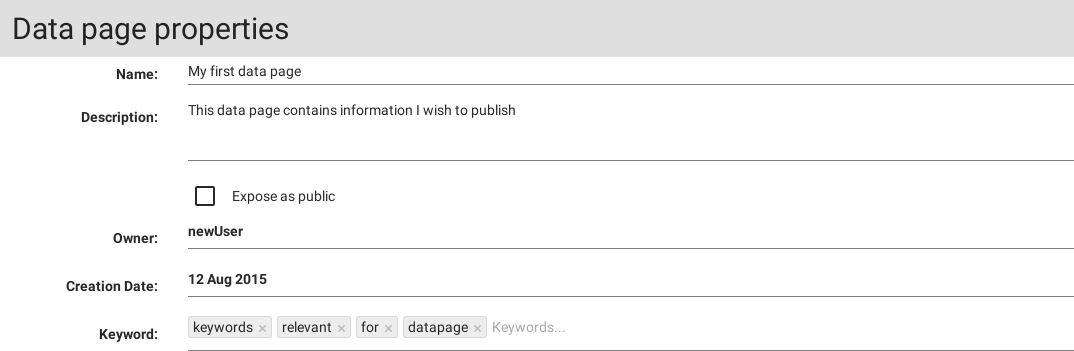
\includegraphics[height=4 cm] {datapagemeta.png}
 \caption{Data page properties \label{datapagemeta}}
\end{figure}
\end{center}

Users that have access to the data page (i.e. just owners in case of private pages and everyone else for public pages) can locally download information associated with a data page in a raw tabular format by pressing {
\includegraphics[scale=0.8]{exportraw.png}} button; or as RDF by pressing {
\includegraphics[scale=0.8]{exportrdf.png}}. The list of supported RDF formats includes RDF/XML(.rdf), n-triple(.nt), turtle(.ttl), n3(.n3), nquads(.nq), RDF/JSON(.rj).
  
%% View portal
%% SPARQL
\subsection{Data transformations}
Another type of asset that users may create and share in DataGraft is data transformation. Before publishing data, in most cases you will need to transform the original dataset -- clean messy data, remove unnecessary information, probably add some new data fields and convert tabular data to RDF. This sequence of operations you perform on your data to convert it to desirable form is called data transformation. The greatest thing about data transformations in DataGraft platform is that you may reuse them repeatably on another datasets, share them with other users, modify existing transformations and create new transformations by extending ones that you or other users created and shared.
As well as data pages, data transformations are stored with some metadata. The transformation properties include transformation name, description, owner and public/private property. They are defined on a data transformation creation stage(see \ref{transform}).

To explore data pages and data transformations created by other users go to the "Explore" tab. Here you can see a list of public assets. 
\section{User Registration}
In order to create your own data pages and transformations through a platform, you should first sign up for DataGraft account. After registration you are automatically redirected to data page creation service, from where you may start a process of creating your first data page. This process is described in detail in section \ref{publish}.

\section{User Dashboard}
User dashboard helps to manage data pages and data transformations created by user.  The dashboard view gives you an overview of your data pages and transformations you have created. 
\section{Publishing data \label{publish}}
Publishing data with help of DataGraft platform is rather simple process. You may start by switching to a {
\includegraphics[scale=0.8]{publish.png}} tab in a main menu. The first thing you do is uploading data. To do so you just drop your dataset file in a raw CSV or RDF format in a white frame under "Upload your data" label. 
\begin{center}
\begin{figure}[!htbp]
\centering
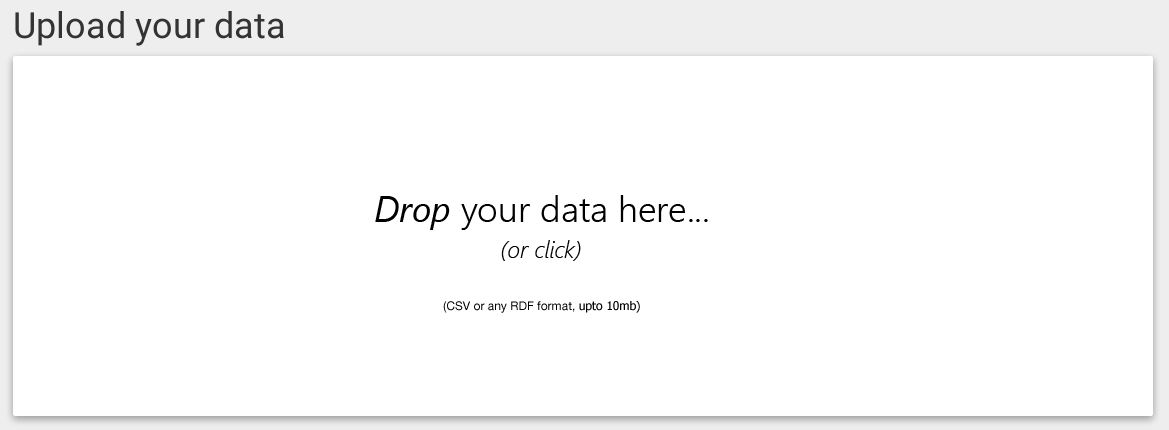
\includegraphics[height=4.5cm] {upload.png}
 \caption{Uploading data \label{meta}}
\end{figure}
\end{center}
After data is succesfully uploaded(this is indicated by green mark in the top right corner of a file icon) you have several options:
	\begin{enumerate}
	\item Create data page from a row data without applying any transformation on it.
	\item Transform your data before creating a datapage. This in turn can be done in two ways	
	\begin{enumerate}
	\item By creating a new transformation to use on your data
	\item By applying an existing transformation to your data
	\end{enumerate}
	\end{enumerate}
	
	
Let's go through the most simple scenario by choosing the first alternative. To do this you just click {
\includegraphics[scale=0.8]{createraw.png}} button. This automatically takes you to the next page where you specify data page properties(see Figure\ref{datapagemeta}). After everything is in order, you simply click {
\includegraphics[scale=0.8]{createdatapage.png}}. And that's it, you have just created your very first data page. Now you (and other users in case if you defined this data page as public) have access to the data page, are able to download associated data, add more information and features to the created asset.

However in most cases you still need to process your data before publishing it. In this case you should use the transformation service. By clicking {
\includegraphics[scale=0.8]{createusingnewtransformation.png}} button you may start transforming your data. Details on how data transformations are created are given in Section \ref{transform}.



\section{Data cleaning and transformation \label{transform}}
This section explains how tabular data is transformed in DataGraft platform and gives you the best strategies for data transformation.

In the basis of DataGraft data transformations there lies a Grafter DSL(Domain Specific Language), which in its turn is implemented in Clojure. Therefore, to take maximum advantage of the service, one should be acquainted with mentioned languages. However number of transformations, depending on their complexity, can be done through intuitive and user-friendly GUI without any coding.



\subsection{Transformation metadata}
The first tab seen in the transformation creation window is "Metadata". Here user defines transformation title and gives a short description of how this transformation processes targeted data. If you wish to share transformation, it is possible to expose it as public. In this case other platform users will be able to explore and use given transformation.


After describing metadata, you may save transformation by clicking “Save” button {
\includegraphics[scale=0.8]{save.png}} in the top right corner. Transformation may be as well saved later at any moment.


\begin{center}
\begin{figure}[!htbp]
\centering
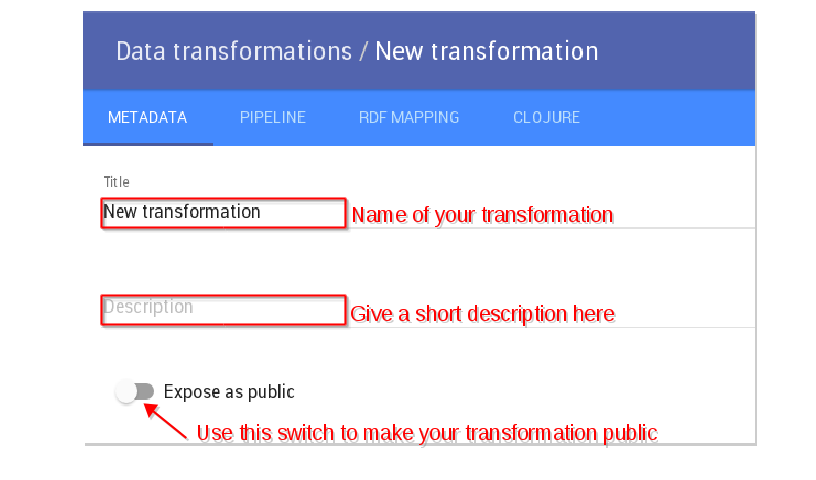
\includegraphics[height=6cm] {transformationmeta.png}
 \caption{Transformation properties \label{meta}}
\end{figure}
\end{center}

\subsection{Transformation Preview}

After your transformation was saved, in the bottom right corner you may see this icon: {
\includegraphics[scale=0.3]{open.png}}. By clicking on it you may immediately apply transformation being created to target data. This may be whether distribution already uploaded to a platform, or alternatively you may upload a new file. For the first option use button depicted as  {
\includegraphics[scale=0.3]{applytoexisting.png}}, and for the second -- this one {
\includegraphics[scale=0.3]{uploadnew.png}}. In this way you are able to see the instant effect of created transformation on your data in the preview area. 

Preview area is located in the right part of transformation window. You can see two tabs there -- one with original data and another with changes made through transformation pipeline. Each time you modify a pipeline, the transformation is  applied to the previewed dataset immediately, so you can see the effect of each performed step. You may adjust preview settings to check and evaluate transformation steps you are creating. Thus, it is possible to hide columns and to sort visible data. The changes made through these settings are not part of transformation and affect just previewed data. However at any time you may export tabular data either as it looks in preview or in a format it has at current stage of your transformation. 

\begin{center}
\begin{figure}[!htbp]
\centering
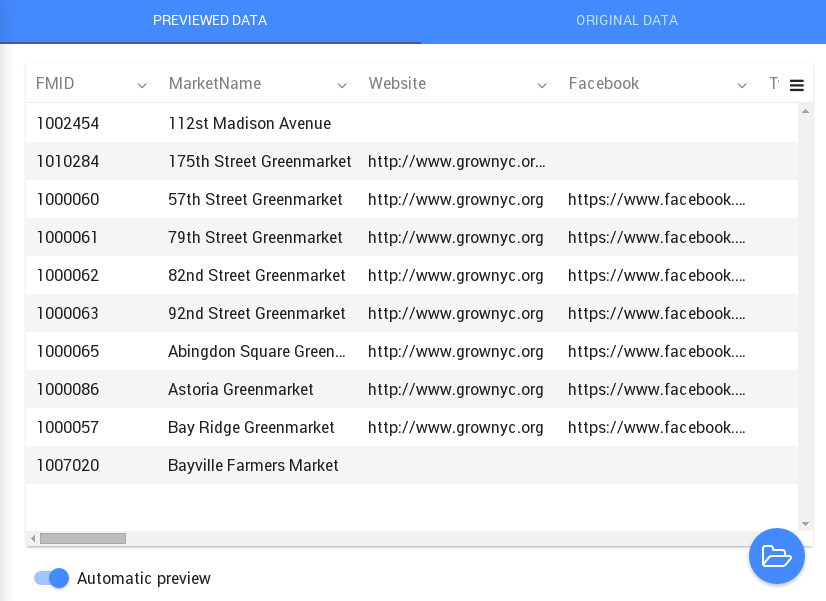
\includegraphics[height=7cm] {preview.png}
 \caption{Transformation preview \label{meta}}
\end{figure}
\end{center}
\subsection{Constructing Transformation Pipeline}
Data cleaning and transformation in DataGraft platform is performed with help of a “pipeline” concept.  To begin with, each single transformation step is defined as a pipe – a function that performs simple data conversion on its input. The greatest fact about these functions is that they may be combined together in a such way, that output of one pipe acts as an input for another. Obviously, the input/output data, that travels through this pipeline is dataset being transformed. This way of composing operations gives a great flexibility and allows to perform rather complex data conversions.

The first implicit step of every transformation pipeline is getting the very first pipeline input. Therefore, each transformation starts from reading a dataset from uploaded file. However you do not need to include this step into your pipeline manually, since this action is performed automatically for each transformation.

To add a first transformation step click the {
\includegraphics[scale=0.5]{add.png}} button next to the pipeline
\begin{center}
\begin{figure}[!htbp]
\centering

\includegraphics[height=2cm] {addpipefunction.png}
 \caption{Add pipe function \label{meta}}
\end{figure}
\end{center}

Now you can see the list of functions you may use to modify uploaded dataset. Available functions are logically grouped according to the type of effect they have on data. Consequently, OPERATIONS ON COLUMNS add, remove or modify dataset columns, while OPERATIONS ON ROWS extract certain rows from a dataset based on row numbers or some condition that user defines. Operations "Make dataset" and "Reshape dataset" affect the entire dataset.
\begin{center}
\begin{figure}[!htbp]
\centering
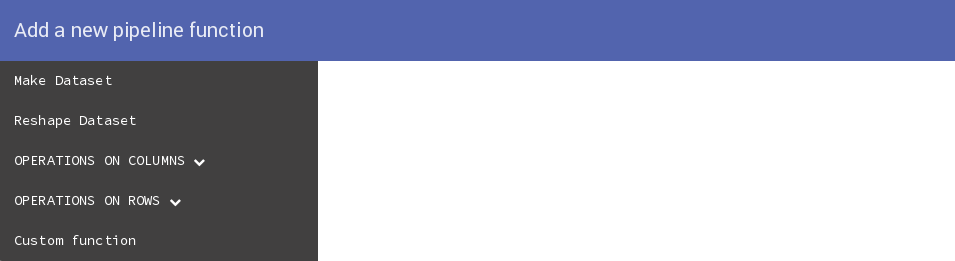
\includegraphics[height=3cm] {functionlist.png}
 \caption{List of available functions \label{meta}}
\end{figure}
\end{center}

 For each operation you can see a short documentation with simple illustrated example by clicking "show/hide documentation" button. For every pipeline function you create you may leave a short description note in the "Comment" field. This information helps you and other users of your transformation to understand operations that are performed here. If you ignore this field, the note will be created automatically based on function parameters you have specified.
 
 \begin{center}
\begin{figure}[!htbp]
\centering
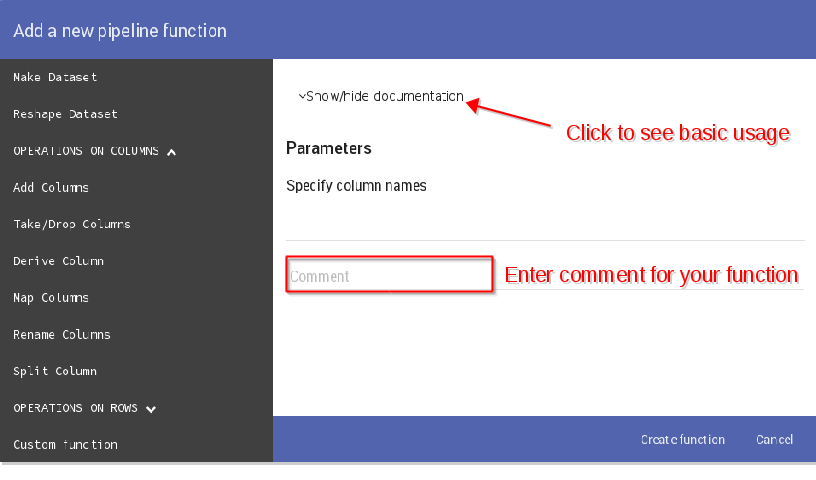
\includegraphics[height=5.5cm] {pipefunccommon1.png}
 \caption{Common operations for all pipe functions \label{meta}}
\end{figure}
\end{center}

Once you have added a new function to the pipeline, it will instantly appear in the pipeline view. You are free to change function parameters any time you need it by simply clicking on correspondent function icon. To get a short information about actions performed by this function you may just hover mouse pointer over its name. In many cases function order significantly affects the transformation result. It is very simple to change this order by just dragging function icons along the pipeline. To remove a function click {
\includegraphics[scale=0.5]{minus.png}} button next to the function you would like to remove.
 
 The following sections provide you with detailed guidelines for each function usage.

  
\subsubsection{Make Dataset \label{makedataset}}
As its name suggests "Make dataset" operation creates new dataset from its input. If you leave all parameter fields blank new dataset will be created from all the input columns with column names given as simple alphabetic sequence. By checking "move first row to header" option you get all the column names from the first row. First row will be removed from your dataset.  You may as well specify column names you wish to see in a new dataset or fetch first n columns.


\subsubsection{Reshape Dataset}
Reshape dataset "melts" given dataset in a such way, that each row of new dataset represents a unique combination of variables and values for given column array. The best way to explain this function is through an example. 

\begin{mdframed}[hidealllines=true,backgroundcolor=blue!20]
%%\begin{example}
{
\includegraphics[scale=0.4]{bulb.png}}
\textcolor{BlueViolet}{\textbf{Example:}}



Let's consider the case, when dataset you are interested in is represented by some sensor measurements data(Figure \ref{ex1_1}).
\end{mdframed}

 \begin{center}
\begin{figure}[!htbp]
\centering
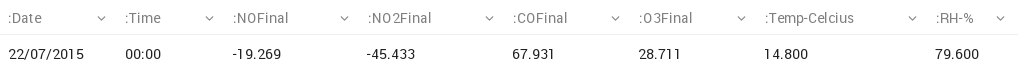
\includegraphics[height=1cm] {ex1_1.png}
 \caption{Original measurement data \label{ex1_1}}
\end{figure}
\end{center}

\begin{mdframed}[hidealllines=true,backgroundcolor=blue!20]
Now you may want to put each measurement into a different row. To do so, you reshape your dataset on fields Date and Time. In this way combination of date and time will be considered as unique id key, while other data will be bound to this key as map of variables and values(see Figure \ref{ex1_4}).
\end{mdframed}

 \begin{center}
\begin{figure}[!htbp]
\centering
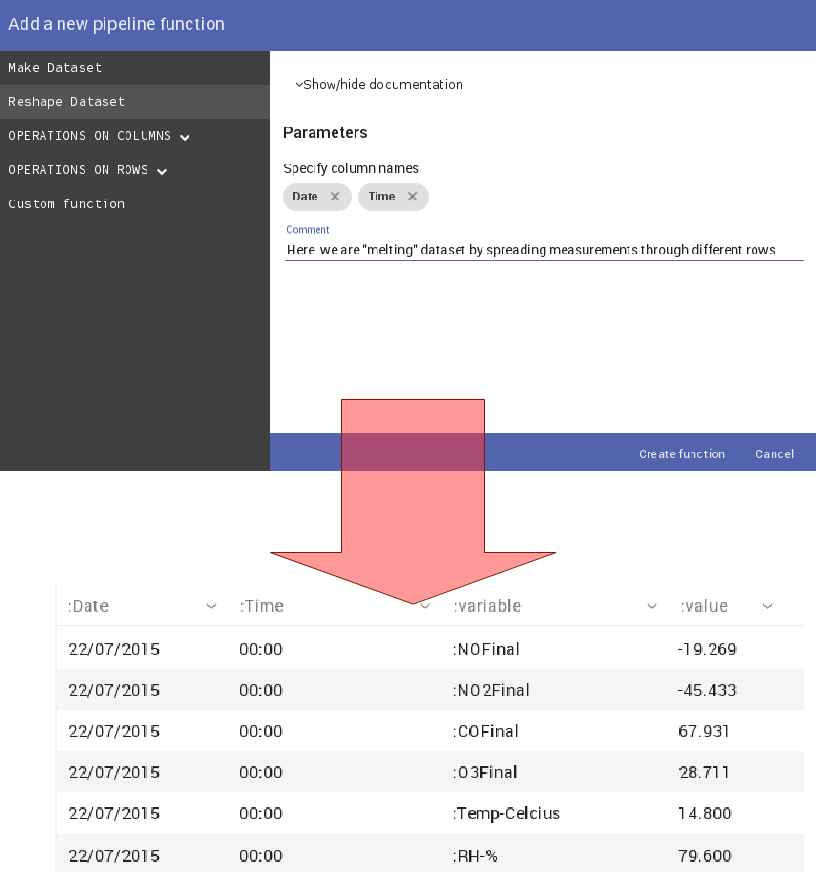
\includegraphics[height=10cm] {ex1_4.png}
 \caption{Reshaped measurement data \label{ex1_4}}
\end{figure}
\end{center}
%%\end{example}






\subsubsection{Add Columns \label{addcolumns}}

The "Add columns"  results in adding a new column(s) to a given dataset. To add a new column you should specify column name and a value for a new column. This value will be copied into every row within dataset. You may as well populate new column with some custom value. This may be current date, dataset filename, row index or custom Clojure code. Note that the "Expression" field is prioritized, in other words if you define both value and expression, only expression will be used to get a value for a new column.
You are able to add as many columns as you need within one operation. To add one more column simply click 

 \begin{center}
\begin{figure}[!htbp]
\centering
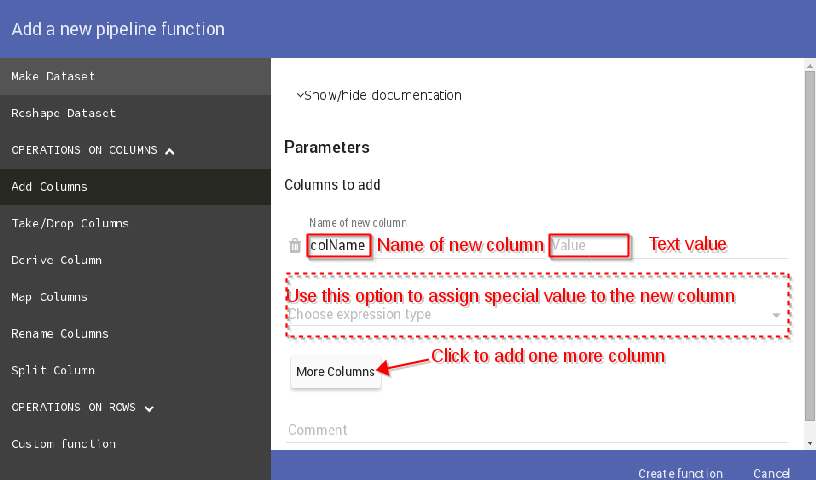
\includegraphics[height=6cm] {addcolumnf1.png}
 \caption{Add Columns function \label{meta}}
\end{figure}
\end{center}


\subsubsection{Take/Drop Columns}

The "Take/Drop Columns" function narrows given dataset. You may explicitly define columns you wish to see in a dataset by listing their names, get first n columns or remove unnecessary columns from a dataset. In a second case, dataset will be narrowed to specified number of columns with their names assigned as alphabletical sequence("A","B","C" etc.). If more than 26 columns are fetched, column names will count "AA", "AB", "AC" ... "BA", "BB", "BC" etc.

 \begin{center}
\begin{figure}[!htbp]
\centering
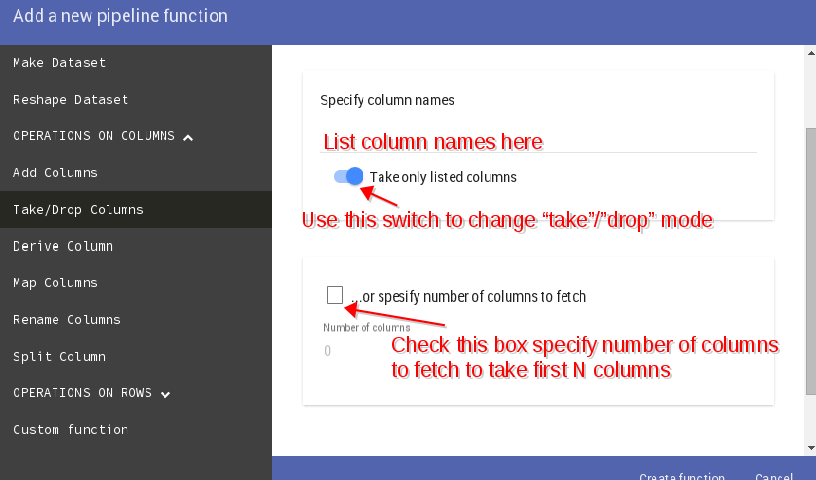
\includegraphics[height=7cm] {columns1.png}
 \caption{Take/Drop Columns function \label{meta}}
\end{figure}
\end{center}

\subsubsection{Derive Column}

This function creates a new column in a dataset by applying some transformation to existing column(or columns). To use this function you should specify name for a new column, define one or several columns you are going to use to obtain new value and specify a function you apply to them. This function can be chosen from a drop-down list, which contains some standard functions and custom utility functions. For your convenience these functions are grouped together based on type of operation they perform. 

If you think that functionality ordered by standard provided functions is not enough to build your transformation, you may define custom utility functions by yourself using Clojure code(see \ref{customFunc}) or use utility functions written by other users. 

Some of functions may expect input parameters in addition to columns, they will operate on. If this is the case, you may specify such a parameter by pressing  {
\includegraphics[scale=0.6]{plus.png}} icon and entering parameter in a field that appears.
\begin{mdframed}[hidealllines=true,backgroundcolor=blue!20]
{
\includegraphics[scale=0.4]{magic.png}}
\textcolor{BlueViolet}{\textbf{Tips and tricks:}}

One powerful feature of derive-column and similar pipeline functions is possibility to combine functions you apply to columns in the same way you combine functions in pipelines. Essentially, these are pipelines inside your dataset manipulation pipeline. To add one more "internal" function into your pipeline function, click {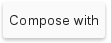
\includegraphics[scale=0.4]{compose.png}} button. Note, that function order is significant in this case. Functions are composed as they appear from top to down. To remove function from composition pipeline click trash icon {
\includegraphics[scale=0.6]{trash.png}} next to the function you wish to delete.
\end{mdframed}


\subsubsection{Map Columns}
This method allows you to apply some transformation to column and put the modified value back to the same column. In parameter list you must specify a column you wish to change and a function that will be used to perform this transformation. You may add as many column-function pairs as you need. 
\begin{mdframed}[hidealllines=true,backgroundcolor=blue!20]
{
\includegraphics[scale=0.4]{magic.png}}
\textcolor{BlueViolet}{\textbf{Tips and tricks:}}

As you probably noticed, the function that appears by default each time you add new mapping pair is string-literal. This function belongs to the group "CONVERT DATATYPE" and plays important role in tabular-to-RDF conversion. 

Whenever you need to treat a column value as a constant literal node, you should first define, which datatype it represents. String-literal will mark  column as one having datatype "string". Another functions used for defining data type are integer-literal and double-literal.
\end{mdframed}

\subsubsection{Rename Columns}
This operation allows you to rename columns in dataset. To get new names for columns you may either apply function(or function pipeline) to current column names or assign mapping from old to new column names directly.

 \begin{center}
\begin{figure}[!htbp]
\centering
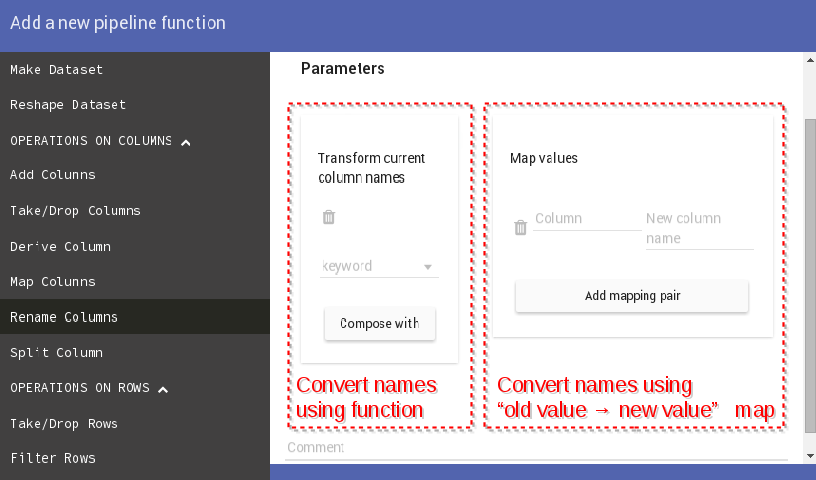
\includegraphics[height=7cm] {renamecolumns1.png}
 \caption{Rename Columns function \label{meta}}
\end{figure}
\end{center}

\begin{mdframed}[hidealllines=true,backgroundcolor=blue!20]
{
\includegraphics[scale=0.4]{magic.png}}
\textcolor{BlueViolet}{\textbf{Tips and tricks:}}

You may see the function named "keyword" assigned by default as a function used to transform column names. This is done because column names in Grafter DSL should be treated as keywords -- special symbolic identifiers used in Clojure language. Having this function as a first one in a list of functions used for column names conversion guarantees column names will be recognized as valid keywords. 
\end{mdframed}

\subsubsection{Split Column}
This operation allows to split column on some separator. Column is splitted once, leaving substring obtained as original text before first instance of separator in the source column and copying text after separator into new column. Separator itself is extracted from text. Name of new column is optional.


\subsubsection{Take/Drop Rows}
This function allows you to take or drop first n rows in a given dataset. Use switch Take rows/Drop rows in the top of the function parameter list to choose between these two options
\subsubsection{Filter Rows}
This method filters rows in the dataset for matches. This is a rather flexible filtering tool that allows you to filter your data in several different ways.

First field in in "Filter Dataset" parameter list specifies whether filter will be applied to specific column(s) or to all columns in dataset. For latter option just leave this field empty and matching will be performed for each column.

To perform actual data filtering you have several options.

First, it is possible to select only rows containing specified text. For this you enter the text in field marked as "Text to match". By default this text is treated as case-sensitive. To perform a case insensitive filtering check the box "ignore case" next to the text field.

You may as well filter dataset with help of regular expressions. By pressing {
\includegraphics[scale=0.6]{tutorial.png}} button next to the "Regular expression" field  you will get short quick start tutorial for pattern usage.

Finally, you may filter dataset by applying utility functions to columns. Note, that the result of function(or combination of functions) will be treated a true/false expression.

The priority of listed option is defined as they appear - from top to down: if "Text to match" field is specified, other fields are ignored, if "Text to match" is ignored, but "Regular expression" is defined -- this one will be used to filter your dataset ignoring functions below(if specified any).

\subsection{Defining Auxiliary Functions \label{customfunction}}

Some complex transformations cannot be done with help of operations described above. In this case you may need to define your own pipeline functions. This can be done with help of "Custom code" option using Clojure language
\subsubsection{Creating and Editing Custom Utility Functions \label{customFunc}}

To create your custom function use {
\includegraphics[scale=0.5]{editutility.png}} button. In window that opens you can see list of available functions at the left side and code editor at the right side.

 \begin{center}
\begin{figure}[!htbp]
\centering
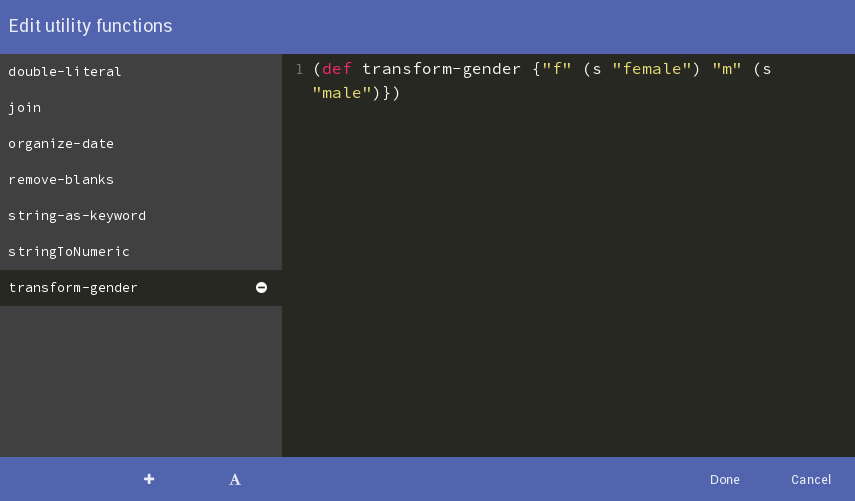
\includegraphics[height=7cm] {createcustom.png}
 \caption{Create custom utility function \label{createutil}}
\end{figure}
\end{center}

Each function can be removed by pressing {
\includegraphics[scale=0.5]{removefun.png}} icon next to the function name. New functions are added by plus icon in the toolbox below function list.

Immediately after you have created a utility function you may start using it as a parameter in pipeline functions.


\begin{mdframed}[hidealllines=true,backgroundcolor=blue!20]
{
\includegraphics[scale=0.4]{magic.png}}
\textcolor{BlueViolet}{\textbf{Tips and tricks:}}

If you create a function having a dataset as an input parameter, it is possible to make it a part of the transformation pipeline directly. You may add this function to a pipeline by choosing "Custom function" option from a pipeline function lists.  

\end{mdframed}


\subsubsection{Creating String Transformation Functions through Graphical Interface \label{customFunc}}

However to specify text transformations you need to perform on your data, you may define new function in a more user-friendly way. To do so press {
\includegraphics[scale=0.5]{createstring.png}} button in the same window, that is used for creating custom utility functions. Now you can see the dialog, where  you specify transformations you want to perform on text values(see Figure \ref{createstring}). All modifications you define are instantly shown with help of sample text at the right bottom corner.

 \begin{center}
\begin{figure}[!htbp]
\centering
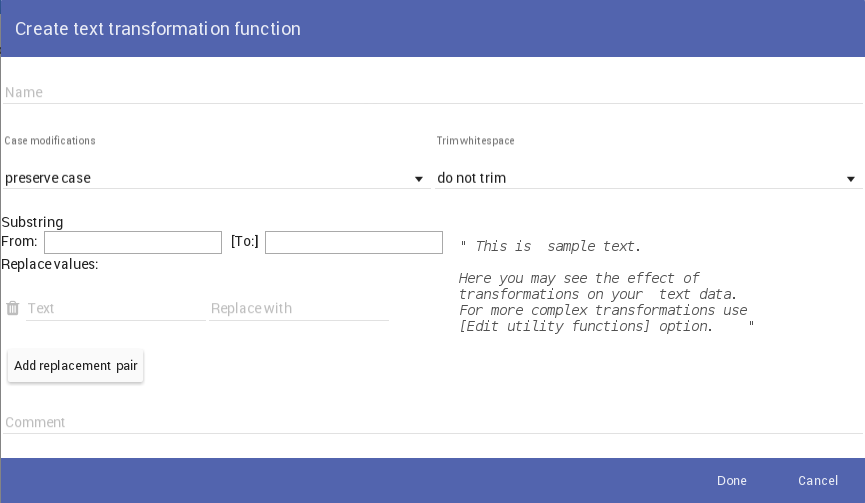
\includegraphics[height=7cm] {createstringwin.png}
 \caption{Create text transformation function \label{createstring}}
\end{figure}
\end{center}


\subsubsection{Creating and Editing Prefixers \label{customFunc}}

You may create and edit prefixers in the "Edit prefixers" window. To see this window  press {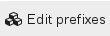
\includegraphics[scale=0.5]{editprefixers.png}} button in the pipeline view. Here you can see the list of all prefixers you created for current transformation. You may add a new prefixer by specifying its name and URI and pressing {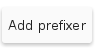
\includegraphics[scale=0.5]{addprefixer.png}} buttom. Created prefixer will instantly appear in the list of prefixers above. It is possible as well to create prefixer by adding some string to the existing one. In this case select a prefixer you wish to choose as base one, enter new prefixer name and string value and press  {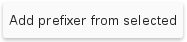
\includegraphics[scale=0.5]{addprefixerfrom.png}}.Now, if the base prefixer is changed, changes will be as well applied to the child prefixers. To remove prefixers select all prefixers you wish to remove and press  {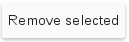
\includegraphics[scale=0.5]{removeprefixers.png}}.

\subsection{Building RDF Mapping \label{customfunction}}

When tabular data is converted to a desirable format, you can start creating RDF mappings. In the process of creating RDF sceleton you can immediately see clear visualization of nodes and corresponding relations.

To start creating RDF mapping of your dataset use switch "Map tabular data to RDF". 
The first step here  would be to specify base graph URI. To create and edit prefixes you are going to need for RDF generation use Edit RDF prefixes button. By pressing it you open a dialog, where you can as well see RDF vocabularies available by default.



%%\begin{mdframed}[hidealllines=true,backgroundcolor=gray!10]
%%\textbf{Example 1.}
%%Here is given a small example, that illustrates how you can transform your data starting from the point where you upload raw csv data and up to the moment where you get the result in desired RDF format.
%%\end{mdframed}




\end{document}